\section{Full real-scan results and qualitative cases}
\label{S-sec:s-results}

\begin{table*}[t]
\caption[Registration recall on nine test cohorts]{Registration recall (\%) on nine test cohorts, including GeoTransformer and ETH inputs beyond \main{\cref*{tab:main}}. ``native'': each frontend's own output. ``F+R'': common training-free verification with finishing of up to 32 candidates followed by the release assay of \main{\cref*{eq:assay}}. Bottom, ``+ learned release'': the optional learned assay, trained on 3DMatch-train. Bold: best and underlined: second best value of the column within each block, at the displayed precision. MAC is the authors' C++ code (\cref{S-sec:s-maccpp}); --: no released ETH setting, and the learned assay was not run on its pools. Each frontend has 16\,GiB and 600\,s per pair, and resource failures count as unregistered pairs. All frontends use the same inputs; the correspondence-based ones run on CPU. \ngr{} and \ls{} are ours, without and with the finite site capacity.}
\label{S-tab:s-main}
\centering\footnotesize
\setlength{\tabcolsep}{4pt}
\ifdefined\supptablebox\else\newsavebox{\supptablebox}\fi
\sbox{\supptablebox}{\begin{tabular}{llrrrrrrrrr}
\toprule
 & & \multicolumn{3}{c}{3DMatch} & \multicolumn{3}{c}{3DLoMatch} & ETH & \multicolumn{2}{c}{KITTI} \\
\cmidrule(lr){3-5}\cmidrule(lr){6-8}\cmidrule(lr){9-9}\cmidrule(lr){10-11}
Frontend & Output & FPFH & FCGF & GeoTr & FPFH & FCGF & GeoTr & FPFH & FPFH & FCGF \\
 & Pairs & 1623 & 1623 & 1623 & 1781 & 1781 & 1781 & 713 & 555 & 555 \\
\midrule
RANSAC-1M & native & 82.3 & 92.5 & \underline{95.4} & 35.1 & 57.9 & 77.4 & 55.8 & \underline{99.6} & \textbf{97.3} \\
 & F+R & 90.2 & \textbf{94.9} & 95.6 & 48.8 & \textbf{67.1} & 78.9 & 89.6 & \textbf{99.8} & \textbf{99.5} \\
\addlinespace[2pt]
SC$^2$-PCR & native & \textbf{83.7} & 92.9 & \textbf{95.6} & 39.0 & 58.3 & 78.1 & \textbf{78.5} & 99.5 & \underline{95.9} \\
 & F+R & \textbf{91.0} & \textbf{94.9} & \underline{96.1} & \underline{52.6} & \underline{67.0} & \textbf{80.3} & \textbf{99.2} & \textbf{99.8} & \underline{99.3} \\
\addlinespace[2pt]
MAC & native & 83.0 & \textbf{93.5} & \textbf{95.6} & 40.0 & \underline{59.0} & \underline{78.3} & -- & \underline{99.6} & 95.7 \\
 & F+R & 90.4 & \underline{94.8} & \textbf{96.2} & 51.6 & 66.4 & \underline{80.2} & -- & \textbf{99.8} & 98.9 \\
\addlinespace[2pt]
TurboReg & native & \textbf{83.7} & \underline{93.3} & \underline{95.4} & 38.5 & 58.7 & 77.9 & 75.9 & \textbf{99.8} & 95.5 \\
 & F+R & 90.4 & \underline{94.8} & \underline{96.1} & 51.5 & 66.1 & 79.8 & 98.0 & \textbf{99.8} & \textbf{99.5} \\
\addlinespace[2pt]
LGR (GeoTr) & native & -- & -- & \underline{95.4} & -- & -- & 77.3 & -- & -- & -- \\
 & F+R & -- & -- & \underline{96.1} & -- & -- & \textbf{80.3} & -- & -- & -- \\
\addlinespace[2pt]
NGR & native & \underline{83.4} & 92.9 & \underline{95.4} & \underline{40.3} & \underline{59.0} & 78.2 & \underline{78.1} & \textbf{99.8} & 95.3 \\
 & F+R & 90.3 & 94.5 & 96.0 & 51.1 & 65.7 & 79.4 & 98.3 & \textbf{99.8} & \underline{99.3} \\
\addlinespace[2pt]
NGRR-LS & native & \underline{83.4} & 93.2 & \textbf{95.6} & \textbf{40.4} & \textbf{59.2} & \textbf{78.6} & \underline{78.1} & \underline{99.6} & 95.3 \\
 & F+R & \underline{90.5} & \textbf{94.9} & 96.0 & \textbf{53.1} & 66.7 & 79.1 & \underline{98.7} & \textbf{99.8} & \textbf{99.5} \\
\midrule
\multicolumn{11}{l}{\emph{Optional learned assay (trained on 3DMatch-train only)}} \\
RANSAC-1M & learned release & 91.9 & 94.9 & 95.6 & 51.4 & \underline{69.5} & 78.8 & 89.8 & \textbf{99.8} & \textbf{99.6} \\
SC$^2$-PCR & learned release & \underline{92.4} & 95.2 & \textbf{96.4} & \underline{55.9} & \textbf{70.2} & \underline{81.1} & \textbf{99.9} & \textbf{99.8} & \textbf{99.6} \\
MAC & learned release & -- & -- & -- & -- & -- & -- & -- & -- & -- \\
TurboReg & learned release & \underline{92.4} & \underline{95.3} & \underline{96.2} & 53.9 & 68.1 & 80.6 & 98.6 & \textbf{99.8} & \underline{99.5} \\
LGR (GeoTr) & learned release & -- & -- & 96.0 & -- & -- & \textbf{81.4} & -- & -- & -- \\
NGR & learned release & 91.3 & 94.5 & 96.0 & 54.0 & 67.5 & 80.0 & 98.7 & \textbf{99.8} & \underline{99.5} \\
NGRR-LS & learned release & \textbf{92.5} & \textbf{95.4} & \underline{96.2} & \textbf{56.2} & 69.1 & 80.1 & \underline{99.3} & \textbf{99.8} & \underline{99.5} \\
\bottomrule
\end{tabular}
}%
\ifdim\wd\supptablebox>\textwidth\resizebox{\textwidth}{!}{\usebox{\supptablebox}}\else\usebox{\supptablebox}\fi

\end{table*}

\paragraph{The authors' C++ MAC.}\label{S-sec:s-maccpp} The MAC results of \main{\cref*{tab:joint,tab:main}}, \main{\cref*{fig:dilute,fig:pareto}} and \cref{S-tab:s-utilization,S-fig:s-results,S-tab:s-main,S-tab:s-cost} use the authors' C++ code with the 12 OpenMP threads it fixes, the same first $\le$5000 correspondences, the 16\,GiB/600\,s limits and the dataset settings of its release, which has none for ETH. On KITTI+FPFH, 25 pairs exceed 16\,GiB; rerun with higher limits, all of them complete (at most 116\,GiB and 1276\,s), so MAC has no unregistered pair from resource limits. Its pool is every hypothesis that MAC computes from its selected cliques, and the common finishing and release are applied unchanged; on 60 evenly spaced 3DLoMatch+FPFH pairs this backend reproduces the stored release of SC$^2$-PCR, with identical poses. The completed width-matched C++ run supplies the frozen synthetic figure and its count-readout control. Our earlier Python adaptation remains in \cref{S-sec:s-synthetic} for decoys, fresh draws and thinned real scans, in the stored pools of \cref{S-sec:s-verification} (release-rule calibration, Top-K and selection-rule comparisons; the main paper reports the latter two without MAC's cells), and in the MAC column of \cref{S-fig:s-qualitative}. Where both complete within the limits (3DMatch+FPFH, 3DLoMatch+FPFH and 3DLoMatch+FCGF), the two implementations register natively within 1.1 points of each other (83.0 against 81.9, 40.0 against 40.4 and 59.0 against 58.8\%). With matched compatibility settings, the checked outcomes agree: on three checked synthetic inputs it gives the same graph, maximal cliques and selected cliques as the authors' code, and on 300 of 300 inputs the same outcome. The authors' code sets this width from the mean point spacing of the clouds it receives, which on the sparse synthetic correspondence sets is about $1.83\tau$, $6.05\tau$ and $0.96\tau$ on cube, sphere and volume, respectively, instead of $0.75\tau$; this explains the lower automatic-scale synthetic recall. The frozen 750-input figure uses the width-matched C++ run; fresh draws, decoys and thinned real scans retain the Python adaptation.

\begin{table*}[t]
\caption[Official criterion]{GeoTransformer's official criterion (registration recall \%, scene mean) on its own correspondences. ``+ finishing'': the finishing step's own choice among up to 32 refined candidates; ``+ release'': the training-free release assay; ``+ learned release'': the optional learned assay. Bold: best per column.}
\label{S-tab:s-official}
\centering\footnotesize
\setlength{\tabcolsep}{4pt}
\begin{tabular}{lrrrrrrrr}
\toprule
 & \multicolumn{4}{c}{3DLoMatch (1726 pairs) $\uparrow$} & \multicolumn{4}{c}{3DMatch (1279 pairs) $\uparrow$} \\
\cmidrule(lr){2-5}\cmidrule(lr){6-9}
Frontend & native & + finishing & + release & + learned release & native & + finishing & + release & + learned release \\
\midrule
RANSAC-1M & 73.55 & 74.49 & 74.55 & 74.58 & 91.50 & 91.90 & 91.93 & 91.90 \\
SC$^2$-PCR & \textbf{74.36} & 75.01 & \textbf{76.02} & 76.35 & \textbf{92.63} & 92.67 & 93.09 & 93.07 \\
TurboReg & 73.57 & 75.15 & 75.93 & 76.42 & 92.09 & 92.59 & 93.09 & 92.64 \\
LGR (GeoTr) & 74.03 & \textbf{75.25} & 75.77 & \textbf{76.51} & 92.48 & \textbf{93.63} & \textbf{93.34} & 93.13 \\
NGR & 74.10 & 74.48 & 75.02 & 75.72 & 92.42 & 92.46 & 92.97 & 92.92 \\
NGRR-LS & 74.33 & 74.56 & 74.84 & 75.83 & 92.30 & 92.62 & 93.10 & \textbf{93.26} \\
\bottomrule
\end{tabular}


\end{table*}

\begin{figure*}[tp]
\centering
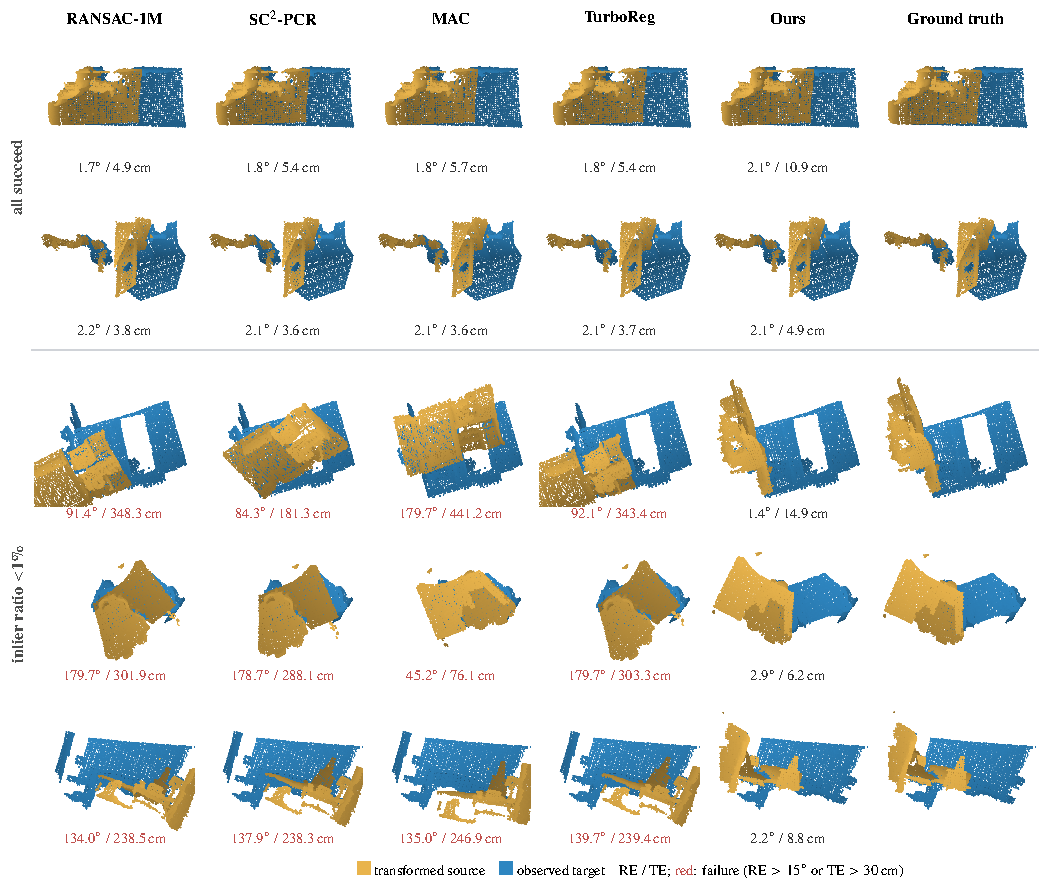
\includegraphics[width=\linewidth]{shared/figures/fig_qualitative.pdf}
\caption[Real cases]{Real cases on 3DLoMatch+FPFH. Gold: source transformed by each method's pose; blue: observed target; one camera and scale per row. Columns 1--4 are each frontend's native output, ``Ours'' is \ls{} with finishing and the training-free release assay. Rows were selected by outcome with a rule fixed before rendering: top, pairs that every method registers (563 pairs), ranked by the number of true inliers; bottom, pairs with an inlier ratio below 1\% on which all four baselines fail and ours succeeds (93 pairs with the earlier MAC adaptation shown in this figure; 97 with the C++ MAC), ranked by target size. Two and three rows were picked for legibility from the first four and six of each list (positions 1 and 2 of the first list; 1, 5 and 6 of the second).}
\label{S-fig:s-qualitative}
\end{figure*}

\paragraph{Paired comparisons.} In \cref{S-tab:s-main}, paired counts $+a/{-}b$ give the pairs registered by the first method but not by the second, and the reverse; $p$ is from McNemar's test~\cite{mcnemar1947}.

On 3DLoMatch+FPFH training-free verification raises recall by 10.8--13.7 percentage points for all six frontends, on 3DLoMatch+FCGF by 6.7--9.2, and on ETH, unseen during design, from 55.8--78.5\% to 89.6--99.2\%. On the saturated cohorts (3DMatch+GeoTr, KITTI+FPFH) the gains stay below one point. No frontend's recall decreases on any cohort.

With the same verification, \ls{} reaches 53.1\% on 3DLoMatch+FPFH, against 52.6\% for SC$^2$-PCR and 51.6\% for MAC. The paired difference from SC$^2$-PCR is not significant (+42/$-$32, $p=0.30$); against MAC it is +55/$-$28 ($p=0.004$). In contrast, \ls{} registers more pairs than \ngr{} (+45/$-$9), TurboReg and RANSAC-1M ($p\le10^{-3}$). On the other FPFH and FCGF cohorts it is within 0.5 points of the best frontend, and over the five frontends evaluated on all nine cohorts its total (9920 pairs) is second to SC$^2$-PCR (9948; +85/$-$113, $p=0.055$).

The optional learned assay adds 1.8--3.3 percentage points on 3DLoMatch with FPFH and FCGF and reaches 56.2\% with \ls{} on 3DLoMatch+FPFH (it was not run on the C++ MAC pools). We selected its features, regularization and weights using only the training cohort, but the 26 candidate features had been listed before the protocol was in place (\cref{S-sec:s-protocol}); we report it separately from the training-free results. Summed over the nine cohorts, the training-free assay obtains 50--58\% of the learned assay's gain over the finishing step's anchor rule for each of the five frontends. Over the nine cohorts, releasing by support alone or by residual shape alone gives 9760 and 9759 registered pairs with \ls{}, against 9920 for their minimum, and for every frontend the minimum releases more pairs than either channel alone.

\paragraph{Scene bootstrap.} Paired gains are more stable than absolute recall, which is estimated from only eight test scenes. A scene bootstrap (2000 resamples of the eight 3DLoMatch test scenes; 95\% intervals) gives 53.1\% [43.9, 60.4] for \ls{} on 3DLoMatch+FPFH, but a gain over its native output of 12.7 [10.3, 14.1] points and over \ngr{} of 2.0 [1.5, 2.5]; against SC$^2$-PCR the difference is 0.6 [$-0.3$, 1.6].

\paragraph{Extremely dilute pairs.} \Cref{S-fig:s-results}(b) and \main{\cref*{fig:dilute}}(a) isolate the 888 3DLoMatch+FPFH pairs with an inlier ratio below 1\%. The native frontends register 26--37 of them. Finishing raises this to 82--124, and the release assay to 106--152, 3.7--5.1 times the native count; the learned assay reaches 148--193 (not run for MAC). With the release assay SC$^2$-PCR registers the most of these pairs (152, against 147 for \ls{}), and the refined pools of the six frontends contain a correct candidate for 169--235 of them. The 381 pairs with only 11--25 true inliers among up to 5000 matches show the same pattern: 7--8 native, 32--38 after finishing and 39--51 after the release assay, where \ls{} registers the most (51). On the 250 pairs with at most ten true inliers every method stays near the floor (3--4 successes without learning, 6--10 with the learned assay).

\paragraph{Qualitative cases.} \Cref{S-fig:s-qualitative} shows real cases. When inliers are plentiful, the methods converge to the same pose. Below 1\% the baselines return poses that are off by 45--180$^\circ$ in the rows shown, while the full pipeline releases a correct candidate. In this cohort 563 pairs are registered by every method, and 93 pairs below 1\% by ours but by none of the four baselines' native outputs (97 with the C++ MAC of \main{\cref*{fig:dilute}}); the illustrations come from these two groups, and the counts above provide the aggregate comparison. The baselines are shown with their native outputs; \cref{S-tab:s-main} and \cref{S-fig:s-results}(b) give their counts with the same verification.

\paragraph{Official criterion.} \Cref{S-tab:s-official} uses GeoTransformer's official criterion (scene mean) on 1726 3DLoMatch and 1279 3DMatch pairs. Its own estimator LGR obtains 74.03\% on 3DLoMatch in our run (74.0\% in~\cite{qin2022geotransformer}); finishing and the release assay raise it to 75.77\%, and the learned assay to 76.51\%. The training-free verification improves every frontend, by 0.5--2.4 percentage points on 3DLoMatch and 0.4--1.0 on 3DMatch. On these learned correspondences, final recall differs by at most 1.5 points across frontends, and \ls{} is not among the best.

\paragraph{Further methods on the same inputs.} \main{\Cref*{tab:main}} adds SC$^2$-PCR++~\cite{chen2023sc2pp}, Regor~\cite{zhao2025regor} and DualReg~\cite{li2026dualreg}, run with their authors' code and per-dataset settings on the same first $\le$5000 correspondences, together with the registration recall and the rotation and translation errors of every frontend. SC$^2$-PCR++ and Regor receive the official keypoint descriptors for their feature-based steps, and DualReg the observed clouds with normals that we estimate from ten nearest neighbors, because the released normals belong to other correspondences; its recall on our inputs is below the published one (37.4 against 41.66\% on 3DLoMatch+FPFH, 94.1 against 98.20\% on KITTI+FPFH). On every cohort the complete pipeline registers at least as many pairs as these three methods, with a lower mean rotation error on the registered pairs.

The complete RR/RE/TE and timing table is in \main{\cref*{tab:main}}. SC$^2$-PCR++ full-cohort accuracy was measured on GPU, while its displayed 0.71\,s is from a separate 16-thread CPU run. On the same 100-pair timing subset the CPU and GPU runs register 45 and 43 pairs, respectively; Its mixed-device point is excluded from the CPU Pareto frontier. Regor uses GPU for both measurements. DualReg timing excludes normal estimation (median 0.026\,s); final release selection adds milliseconds beyond the timed moments.
